\subsection{Feature evaluation} \label{sec:body_feature_evaluation}

Concluding chapter \ref{sec:body_relevant_features} I have identified the following features that describe effective mnemonics. 
\begin{enumerate}
    \item word vividness (imageability, concreteness)
    \item bizarreness of mental imagery
    \item centrality of input words with strong connections in the output
\end{enumerate}

Given the existing research it is plausible to start with quantifying the vividness of the mnemonics. It would be perhaps most plausible to train a model that outputs a score that captures the vividness of the input text. Unfortunately I was unable to find such data. In the field of psycho-linguistics however norms of words exist. Several datasets are available that incorporate human word scores for different norms. Norms relevant to my research are: imageability, concreteness and sensory modality. The latter seems useful as words that are strongly identified with different senses are likely to be very concrete and contribute to vivid imagery. One limitation that quickly emerges is that these datasets tend to be rather small and using them on their own won't cover enough words to be used effectively. Several successful attempts have been made to extend these norm datasets by training models that identify features from word embeddings \cite{concr_embed_bert, img_concr_svm, fusing_ctx_embed_concr}. \cite{concr_embed_bert} referred to research showing that concrete word embeddings tend to cluster with other concrete ones while abstract ones show the same general behavior. This is not surprising as embeddings from increasingly sophisticated models encode features of text extracted from enormous corpora. I mostly copied the architecture described in their paper to fine-tune DistilBERT for the regression task of predicting a concreteness scalar $c \in [0,1]$. In addition to the generous dataset of 40000 human concreteness ratings \cite{40000_concr} I trained the model with another 60000 multi word expressions from \cite{60000_concr}. This allows me to evaluate phrases rather than just words of the mnemonics in terms of concreteness. The fine-tuned model achieved a Pearson correlation of $0.88$ with the test data. Ten percent of the dataset had been used for testing. While this result is good the models of the paper performed up to $0.92$ in correlation. This gap in performance could be explained by the additional dataset used on my part. I suspect that it becomes less trivial to assess concreteness adding multi-word expressions to the training data. To support that point I have fine-tuned BERT as described in the paper with just using the 40000 word ratings. This model achieved a Pearson correlation of $0.918$ which is close enough. On a side note I hypothesized that more recent models like CLIP are perhaps better suited for the task of predicting concreteness as they form embeddings from text combined with images. My idea is that more abstract terms are in a different embedding space than concrete ones because they tend to have less distinct images associated with them. The set of possible images for the word \emph{cow} is probably a lot smaller than for the word \emph{female}. To investigate this I've compared CLIP with BERT on predicting word concreteness. Two models for each architecture had been trained. One that fine-tuned all weights while the other one froze all weights except for the regression head. This gives us an idea of how well the raw embeddings are at predicting concreteness. It may have been more appropriate to use imageability ratings for this comparison but since imageability and concreteness are related and the existing data for the latter is far more abundant, I chose to use concreteness ratings for this task. 
\begin{table}[ht]
\centering
\begin{tabular}{@{}lcc@{}}
\toprule
Model & Unfrozen Weights & Frozen Weights \\ \midrule
BERT           & 0.918                     & 0.752                   \\
CLIP           & 0.905                     & 0.800                   \\ \bottomrule
\end{tabular}
\caption{Pearson correlations for BERT and CLIP with unfrozen and frozen weights.}
\label{tab:clip_bert_comparison}
\end{table}
As expected (see Table \ref{tab:clip_bert_comparison}) the CLIP model with frozen weights outperformed the BERT version, however it strikes me as surprising that the opposite effect was observed in the case of fine-tuning all weights. This may be explained due to architecture differences and would require further research.

Two more DistilBERT models have been fine-tuned to predict imageability and sensory modality scores. The latter was trained with 1792 examples \cite{Juhasz2013} gathered from participants that where asked to rate the degree to which each word evoked a sensory experience. The MRC psycholinguistic database \cite{mrc} contains 4828 imageability ratings which I used to train the first model. The models used for evaluating mnemonics and their test results are displayed in Table \ref{tab:linguistic_features_pearsonr}.


\begin{table}[ht]
\centering
\begin{tabular}{@{}lc@{}}
\toprule
Models          & Pearson Correlation \\ \midrule
Concreteness             & 0.880                        \\
Sensory Modality         & 0.706                        \\
Imageability             & 0.875                        \\ \bottomrule
\end{tabular}
\caption{Pearson correlation coefficients for the fine-tuned DistilBERT models}
\label{tab:linguistic_features_pearsonr}
\end{table}
Perhaps the most straightforward way to evaluate the mnemonics is to take the mean (Equation \ref{eq:token_mean}) of the word scores from the individual models.
\begin{equation} \label{eq:token_mean}
    s_{\text{mnemonic}} = \frac{1}{N}\sum_{w=1}^{N}\text{model}(w)
\end{equation}
I consider only words that are not labeled as stopwords. The results for sensory modality, imageability and concreteness are shown in Tables \ref{tab:mean_std_ser}, \ref{tab:mean_std_img}, \ref{tab:mean_std_concr} and Figures \ref{figure:ser_mean_box_plot}, \ref{figure:img_mean_box_plot}, \ref{figure:concr_mean_box_plot} respectively.
\begin{table}[ht] 
\centering
\caption{Means and Standard Deviations for Sensory Modality}
\label{table:group_stats}
\begin{tabular}{lcc}
\toprule
Group & Mean & Standard Deviation \\
\midrule
GPT-2& $0.337$ & $0.043$ \\
GPT-3 (mnemonic) & $0.320$ & $0.055$ \\
GPT-3 (paragraph)& $0.351$ & $0.065$ \\
WaniKani & $0.347$ & $0.063$ \\
\bottomrule
\end{tabular}
\label{tab:mean_std_ser}
\end{table}

\begin{table}[ht] 
\centering
\caption{Means and Standard Deviations for Imageability}
\label{table:group_stats}
\begin{tabular}{lcc}
\toprule
Group & Mean & Standard Deviation \\
\midrule
GPT-2& $0.558$ & $0.043$ \\
GPT-3 (mnemonic) & $0.569$ & $0.054$ \\
GPT-3 (paragraph)& $0.583$ & $0.065$ \\
WaniKani & $0.582$ & $0.063$ \\
\bottomrule
\end{tabular}
\label{tab:mean_std_img}
\end{table}

\begin{table}[ht] 
\centering
\caption{Means and Standard Deviations for Concreteness}
\label{table:group_stats}
\begin{tabular}{lcc}
\toprule
Group & Mean & Standard Deviation \\
\midrule
GPT-2& $0.558$ & $0.043$ \\
GPT-3 (mnemonic) & $0.569$ & $0.054$ \\
GPT-3 (paragraph)& $0.583$ & $0.065$ \\
WaniKani & $0.582$ & $0.063$ \\
\bottomrule
\end{tabular}
\label{tab:mean_std_concr}
\end{table}

\begin{figure}
    \centering
    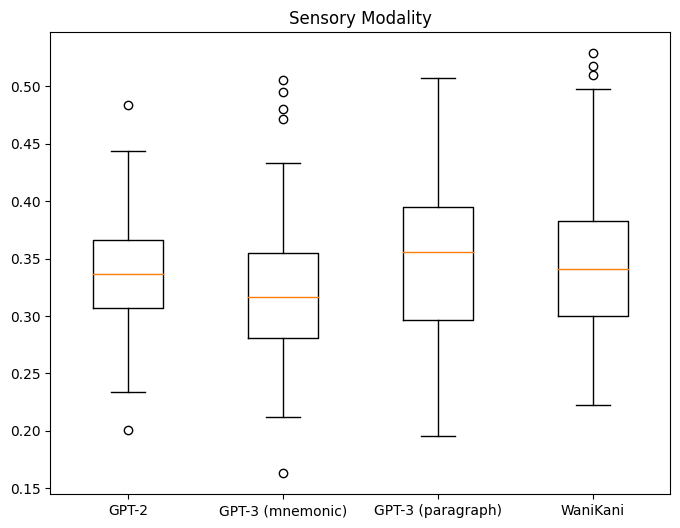
\includegraphics[width=400pt]{resources/ser_mean_box_plot.png}
    \caption{Sensory Modality Mean Scores}
    \label{figure:ser_mean_box_plot}
\end{figure}

\begin{figure}
    \centering
    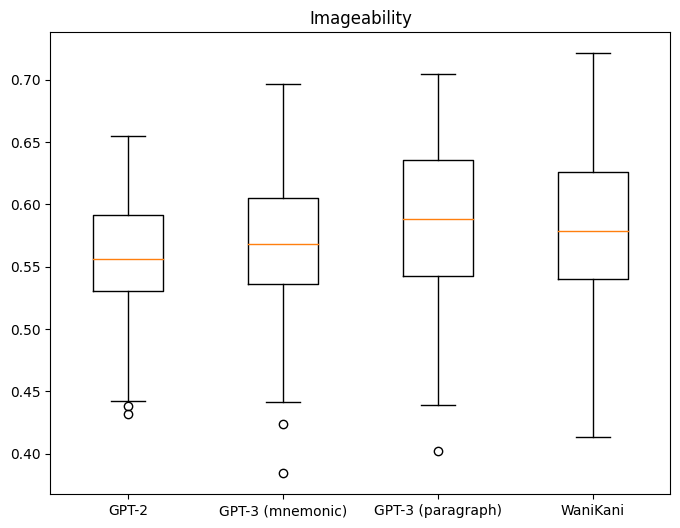
\includegraphics[width=400pt]{resources/img_mean_box_plot.png}
    \caption{Imageability Mean Scores}
    \label{figure:img_mean_box_plot}
\end{figure}

\begin{figure}
    \centering
    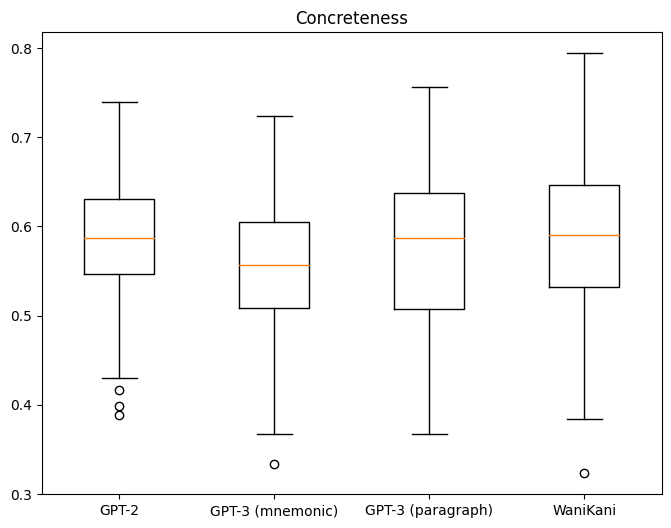
\includegraphics[width=400pt]{resources/concr_mean_box_plot.png}
    \caption{Concreteness Mean Scores}
    \label{figure:concr_mean_box_plot}
\end{figure}
The ANOVAS's for all features were significant ($p < 0.05$). However, the differences are not very striking and the significant interaction terms between groups often show the opposite trend of what I had hoped for. Namely the paragraphs from GPT-3 often and GPT-2 generated mnemonics often have a higher overall mean than GPT-3 mnemonics and the WaniKani mnemonics. I have also tried to use the $median$ and $maximum$ of mnemonic scores but the results are comparable and therefore of no further interest. Given these results I conclude that simple metrics like $mean$, $median$, and $maximum$ of language norm scores over all tokenized words of individual mnemonics aren't very useful in separating the groups.

As a next step I want to quantify the bizarreness of text to potentially separate the four groups. Based on the observation that bizarre language uses words that are not commonly found together we may get some estimate of how bizarre a mnemonic is, based on the probability of their content occurring. To clarify this the phrase "a horse and a tiger racing each other" is probably a lot less likely to occur than seeing the phrase "two cars racing each other". To get a value for how likely text is to occur I will use perplexity scalars. This metric was explained earlier in Chapter \ref{sec:body_state_of_the_art} (Equation \ref{eq:ppl}). One reason to be careful with this metric is that its measures are dependant on the training data and model architecture. For the experiment I used GPT-2 based perplexity which was trained with a dataset called WebText which was never fully published but contains mostly text from web pages that had been scraped by following outbound links from Reddit \cite{gpt2_hugging_face}. Results are shown in Table \ref{tab:ppl_whole_mnemonic} and plotted in Figure \ref{figure:ppl_whole_mnemonic}.     
\begin{table}[ht] 
\centering
\caption{Means and Standard Deviations for Perplexity}
\label{table:group_stats}
\begin{tabular}{lcc}
\toprule
Group & Mean & Standard Deviation \\
\midrule
GPT-2& $20.08$ & $12.71$ \\
GPT-3 (mnemonic) & $13.08$ & $4.30$ \\
GPT-3 (paragraph)& $22.63$ & $16.18$ \\
WaniKani & $36.13$ & $18.08$ \\
\bottomrule
\end{tabular}
\label{tab:ppl_whole_mnemonic}
\end{table}
\begin{figure}
    \centering
    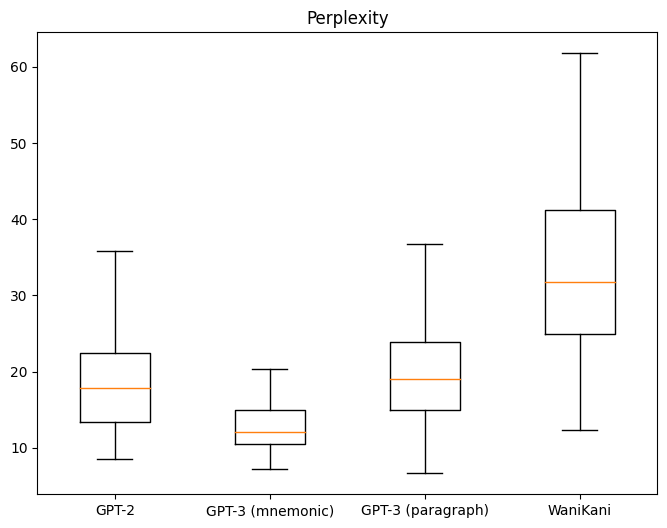
\includegraphics[width=400pt]{resources/ppl_entire_mnemonic.png}
    \caption{Perplexity Values}
    \label{figure:ppl_whole_mnemonic}
\end{figure}

As is evident, the ANOVA was highly significant ($p = 0.000$). We can also observe the promising clear shift between WaniKani mnemonics and all other groups. The difference between the GPT-2 XL mnemonics and the WaniKani ones, however, is alarming. Given that the former frequently contains incoherent phrases due to the beam search constrains, I would have expected their perplexity values to be much higher. Additionally the GPT-3 mnemonics have the overall lowest perplexity which renders the utility of perplexity for evaluating mnemonics questionable. The mnemonics by GPT-3 are storylike and often start with "Once upon a time". Perhaps the relatively low perplexity can be explained by taking a deeper look at the training data. It is possible that WebText contained a lot of story material. Moreover, the result may be explained by the model favoring output from other AI models over text written by humans. This poses an interesting question about the limitations of current language models that could be examined further. 

In order to reduce the overall bias towards different structures of text I chose to do second experiment. Instead of computing perplexity for the entire mnemonic, I tokenized the text into chunks of roughly $4$ words and then considered their mean. (Table \ref{tab:ppl_4_chunks}, Figure \ref{figure:ppl_4_chunks}) I should mention that for the Figures showing perplexity, outliers have been removed.
\ref{figure:ppl_4_chunks}.     
\begin{table}[ht] 
\centering
\caption{Means and Standard Deviations for Perplexity (Chunks)}
\label{table:group_stats}
\begin{tabular}{lcc}
\toprule
Group & Mean & Standard Deviation \\
\midrule
GPT-2& $2734$ & $6373$ \\
GPT-3 (mnemonic) & $703$ & $741$ \\
GPT-3 (paragraph)& $629$ & $361$ \\
WaniKani & $956$ & $592$ \\
\bottomrule
\end{tabular}
\label{tab:ppl_4_chunks}
\end{table}
\begin{figure}
    \centering
    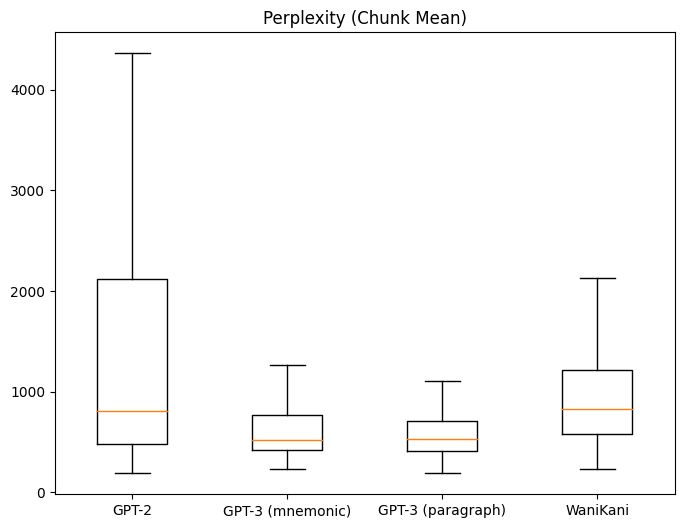
\includegraphics[width=400pt]{resources/ppl_4_chunks.png}
    \caption{Perplexity Values (Chunks)}
    \label{figure:ppl_4_chunks}
\end{figure}

The results turn out to be much more promising for the second attempt. As expected perplexity for GPT-2 mnemonics is now enormous and Wankani mnemonics are much more "perplexed" than the GPT-3 ones. Although not significant at all the mean of the GPT-3 mnemonics is now slightly higher than that of the paragrah ones. Overall, these numbers support the idea that perplexity is related to the bizarreness of language and should be considered to be included in the final metric. 





